\documentclass[bachelor, och, labwork]{shiza}

\usepackage[utf8]{inputenc}
\usepackage{graphicx}

\usepackage[sort,compress]{cite}
\usepackage{amsmath}
\usepackage{amssymb}
\usepackage{amsthm}
\usepackage{fancyvrb}
\usepackage{longtable}
\usepackage{array}
\usepackage[english,russian]{babel}
\usepackage{minted}

\usepackage{tempora}


% \usepackage[colorlinks=false]{hyperref}


\newcommand{\eqdef}{\stackrel {\rm def}{=}}


\begin{document}

\title{Алгоритмы алгебры и теории чисел}

\course{4}

\group{431}

\napravlenie{10.05.01 "--- Компьютерная безопасность}


\author{Никитина Арсения Владимировича}


\satitle{доцент}
\saname{А.\,С.\,Гераськин}


\date{2022}

\maketitle

% Включение нумерации рисунков, формул и таблиц по разделам
% (по умолчанию - нумерация сквозная)
% (допускается оба вида нумерации)
%\secNumbering


\tableofcontents

\section{Задание лабораторной работы}

Осуществить проверку чисел на простоту с помощью критерия Вильсона.

\section{Теоретическая часть}

\begin{center}
    Теорема Вильсона
\end{center}

Если $p$ --- простое число, то выполняется соотношение $(p-1)!+1\equiv 0~(mod~ p)$, 
а если $p$ -- составное, то соотношение не выполняется.

Для доказательства потребуется вспомогательное утверждение: 

Если НОД($a,b$) = 1, то $\exists u,v\in \mathbf{Z} : au + bv = 1$.

Итак, докажем теорему.

Очевидно, достаточно доказать утверждение для случая, когда $a, b$ --- натуральные 
числа. Нетривиальной частью доказательства является идея индукции по сумме $a+b$. 
При $a+b=2$ имеем $a=b=1$ и $au + bv = 1$ выполняется с $u=1$, $v=0$. Пусть 
теорема верна для всех $a, b:$ НОД(a,b)=1, $a+b<k$, где $k>2$. Тогда, так как $a+b>2$, 
НОД(a,b)=1, то $a \not=b $. Не теряя общности можно считать, что $a>b$. 
Поскольку, очевидно, НОД(a-b,b)=1 и $(a-b)+b=a<k$, по индуктивному предположению 
существуют целые $x, y$, такие, что:

\begin{center}
    $(a-b)x+by=1$ или $ax+b(y-x)=1$.
\end{center}

Положив $x=u$, $y-x=v$, получим $au + bv = 1$, что и требовалось доказать.


\section{Практическая часть}
\subsection{Пример работы алгоритма}
\begin{figure}[H]
    \centering
    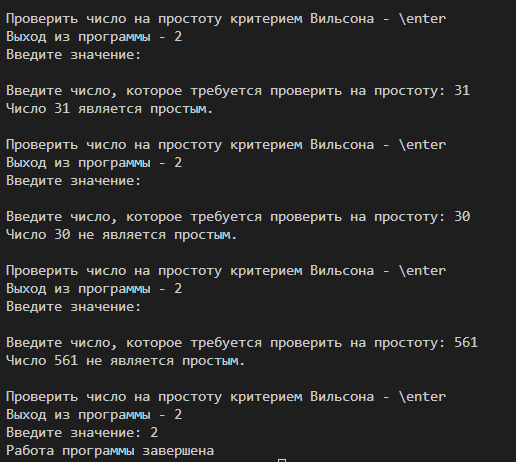
\includegraphics[width=0.8\textwidth]{pic1.png}
    \caption{}
\end{figure}

\setminted[python]{linenos,breaklines=true, fontsize=\small, style=bw}
    \subsection{Код программы, реализующей рассмотренный алгоритм}
        \inputminted{python}{lab3.py}

\end{document}